% Fig. 4.8 / CH4_FIGURE_SPECS.md -- two Student t densities carrying the same
%   right-tail probability, so that the tail point of the larger degree of
%   freedom is seen to be the smaller of the two.
% Source: mathstatch4.tex lines 4230-4272 (the tikzpicture of the Note that
%   follows the 中央工管 multiple-choice item).  The manuscript draws it with
%   pgfplots: two \addplot curves, student(x,1) solid and student(x,10)
%   dashed, over domain -6:6 with samples=400, axis ranges xmin=-6.2,
%   xmax=6.2, ymin=0, ymax=0.45, only the bottom axis line drawn
%   (axis y line=none), no y tick labels, and three x ticks at
%   0, 1.517898 and 3.894743 labelled $0$, $t_{\alpha}(10)$ and
%   $t_{\alpha}(1)$.  Two gray tails at opacity 0.1 (under t(1) from 3.894743
%   to 6, under t(10) from 1.517898 to 6) and two boundary segments dropped
%   from the curves to the axis at those two abscissae, solid for t(1) and
%   dashed for t(10).  The x axis is named $t$.
%
% The two densities, both written out in closed form so that no gamma
% function has to be evaluated at run time:
%   t(1)  = standard Cauchy:  f(x) = 1/(pi(1+x^2)) = 0.31830989/(1+x^2)
%   t(10):                    f(x) = 0.38910838 (1+x^2/10)^{-11/2}
%           the constant is Gamma(11/2)/(sqrt(10 pi) Gamma(5))
%           = 52.342778/(5.6049912 x 24).
% The heights the manuscript hard-codes for the two boundary segments follow
% from these: f_{t(1)}(3.894743) = 0.0196864 and f_{t(10)}(1.517898) =
% 0.1243979, both reproduced to seven places.  The common right-tail
% probability is 0.0797, which the manuscript does not print on the figure;
% it is not printed here either.
%
% Departures from the manuscript figure, all of them required by the site
% specs:
%
% 1. Colour and line width per CH3_FIGURE_SPECS 1: curves and axis in
%    journalink at 0.8pt, tails in journalaccent at fill opacity 0.15 rather
%    than gray at 0.1.
%
% 2. The manuscript lets the two gray tails overlap on [3.894743, 6], where
%    the shading comes out twice as dark for no reason of its own.  CH2 spec
%    1.2 forbids building tone by superposition, so the two fills here are cut
%    to disjoint pieces of the same union: the whole area under t(10) from
%    1.517898 to 6, and the strip between t(10) and t(1) from 3.894743 to 6.
%    The union drawn is exactly the manuscript's union, at one even tone.
%
% 3. The tick label $0$ is set on a second row.  On one row the box of
%    $t_{\alpha}(10)$ stands 0.344cm clear of the box of $0$, under the 0.6cm
%    of CH2 spec 1.3; the two tail-point labels, which are the ones the figure
%    is about, then clear each other by 0.628cm on the row they share.
%
% 4. The manuscript's \addlegendentry pair becomes a two-row legend in the top
%    right corner with 0.5cm samples, as in kurtosis-tail-comparison.tex.
%    Direct labels at the curves are not usable: the two lie within 0.06 of
%    each other in density over the whole of |x| > 2.4.
%
% Size and type.  Drawing range 8.19cm wide, inside the 9.0cm cap of CH2 spec
% 1.3.  A mark of S pt shows at S x 0.99626 x <display width> / <native width>
% px.  The figure sits inside a Note box, where a topic-figure--wide is
% 309px on a 390px phone and 602px on the desktop; the smallest mark in the
% picture is the alpha of $t_{\alpha}(10)$, at script size, which
% \DeclareMathSizes{10}{10}{9}{8} holds at 9pt rather than the 7pt of the
% default math sizes.
\documentclass[tikz,border=2pt]{standalone}
\usepackage{amsmath}
\usepackage{amssymb}
\usepackage{xcolor}
\usetikzlibrary{arrows.meta}
\DeclareMathSizes{10}{10}{9}{8}

\definecolor{journalink}{HTML}{1F1C18}
\definecolor{journalmuted}{HTML}{8A7F72}
\definecolor{journalaccent}{HTML}{9C2D2D}

\newcommand{\tone}[1]{0.31830989/(1+(#1)*(#1))}
\newcommand{\tten}[1]{0.38910838*pow(1+(#1)*(#1)/10,-5.5)}

\begin{document}
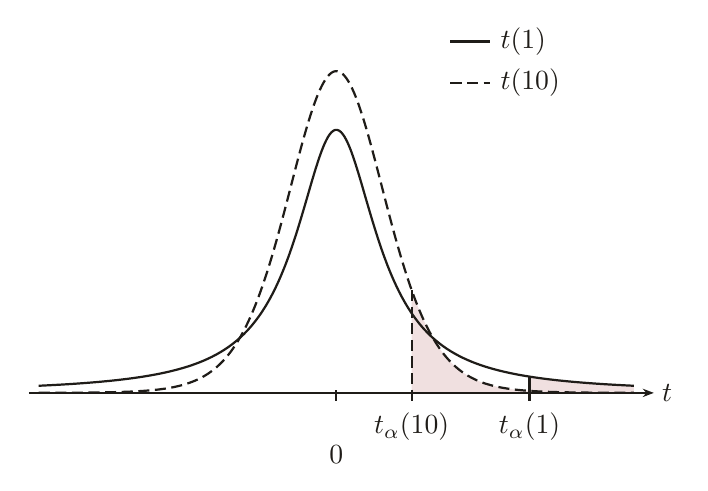
\begin{tikzpicture}[
  x=0.63cm,
  y=10.5cm,
  every node/.style={font=\normalsize, journalink},
  axis/.style={journalink, line width=0.8pt, -{Stealth[length=4pt]}},
  tick/.style={journalink, line width=0.8pt},
  curveone/.style={journalink, line width=0.8pt},
  curveten/.style={journalink, line width=0.8pt,
                   dash pattern=on 4pt off 2pt},
  tail/.style={journalaccent, fill opacity=0.15}
]
  % ---- the two shaded tails, cut so that they do not overlap -----------
  % All of the area under t(10) from its tail point out to the right edge.
  \fill[tail] (1.517898,0) -- (6,0) -- (6,0.0000881)
    -- plot[domain=6:1.517898, samples=220, smooth] (\x,{\tten{\x}})
    -- cycle;

  % The strip between t(10) and t(1) from the tail point of t(1) rightwards;
  % together with the piece above, this is the area under t(1) on the same
  % interval.
  \fill[tail] (3.894743,0.0024283)
    -- plot[domain=3.894743:6, samples=140, smooth] (\x,{\tten{\x}})
    -- (6,0.0086030)
    -- plot[domain=6:3.894743, samples=140, smooth] (\x,{\tone{\x}})
    -- cycle;

  % ---- the two densities -----------------------------------------------
  \draw[curveone] plot[domain=-6:6, samples=320, smooth] (\x,{\tone{\x}});
  \draw[curveten] plot[domain=-6:6, samples=320, smooth] (\x,{\tten{\x}});

  % ---- x axis -----------------------------------------------------------
  \draw[axis] (-6.2,0) -- (6.4,0);
  \node[anchor=west, inner sep=2.8pt] at (6.4,0) {$t$};

  % ---- the two tail points ----------------------------------------------
  % Each boundary segment takes the line style of the curve it comes down
  % from, as in the manuscript.
  \draw[curveone] (3.894743,0.0196864) -- (3.894743,0);
  \draw[curveten] (1.517898,0.1243979) -- (1.517898,0);

  \foreach \p in {0, 1.517898, 3.894743}
    \draw[tick] ([yshift=0.035cm]\p,0) -- ([yshift=-0.106cm]\p,0);

  % Upper row: the two tail points, whose boxes are 0.479cm and 0.390cm wide
  % either side of centres 1.497cm apart, so they clear each other by
  % 0.628cm.  Lower row: the origin.
  \node[anchor=north, inner sep=0pt] at ([yshift=-0.25cm]1.517898,0)
    {$t_{\alpha}(10)$};
  \node[anchor=north, inner sep=0pt] at ([yshift=-0.25cm]3.894743,0)
    {$t_{\alpha}(1)$};
  \node[anchor=north, inner sep=0pt] at ([yshift=-0.66cm]0,0) {$0$};

  % ---- legend, top right corner -----------------------------------------
  % Rows at 4.4625cm and 3.9375cm above the axis, i.e. at densities 0.425 and
  % 0.375; neither curve reaches 0.06 anywhere to the right of x = 2.3, so
  % both rows stand well clear.  Samples 0.5cm long per CH2 spec 1.9.
  \draw[curveone] ([yshift=4.4625cm]2.30,0) -- ([yshift=4.4625cm]3.0937,0);
  \node[anchor=west, inner sep=0pt] at ([yshift=4.4625cm]3.30,0) {$t(1)$};

  \draw[curveten] ([yshift=3.9375cm]2.30,0) -- ([yshift=3.9375cm]3.0937,0);
  \node[anchor=west, inner sep=0pt] at ([yshift=3.9375cm]3.30,0) {$t(10)$};
\end{tikzpicture}
\end{document}
